Firstly, this paper tackles the problem of specifying high-level robot tasks in a way compatible with the open world assumption. Then, we consider the need for re-planning, which arises when new elements of the open world are introduced. We begin by stating what is meant by \emph{open world} in the current context; that of controller synthesis.

\begin{myDefinition}
	\textbf{(Open World):} The union of $\mathcal{X}$ and $\mathcal{Y}$, the sets of environment and robot proposition respectively, defines the state-space. If the state-space is allowed to increase and decrease in size during execution, then we say that the robot operates in an open world.
\end{myDefinition}
\ldots We will return to this definition in Section \ref{openworld}.
%We are mostly concerned with increasing state-spaces, which arise in scenarios where new elements of a mission are introduced during execution.

The need to express mission specifications differently when the robot is expected to operate in an open world is motivated by real-world applications, such as autonomous search and rescue scenarios. In such cases, the mission has to be specified before the robot has obtained full knowledge of the world. In other cases, the state-space may be (i) too large for the user to enumerate every possible variation upfront, and/or (ii) too large for the synthesis algorithm to process. To clarify the latter cases, consider the following scenario:
% FIXME: The paper doesn't actually address (ii). The state-space will still get too large for synthesis.
% FIXME: Make the 3 motivation (i), (ii), (iii). Then I can refer to them properly.

\begin{myExample}\label{Ex:mailbot1} Autonomous Mailbot\\
	A robotic courier (mailbot) operates within a school or company building. It is tasked with collecting letters and delivering them to the offices of the corresponding recipients. Even if all possible recipients and the locations of their offices are known, the information may not be available at the time the mission specification is defined. 
\end{myExample}

\begin{figure}[ht]
	\centering
	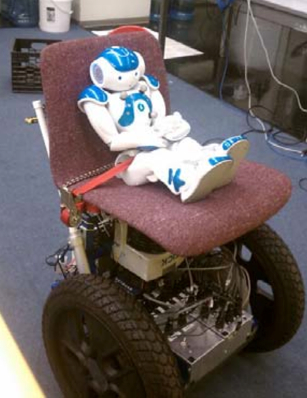
\includegraphics[width=0.7\columnwidth, clip]{./img/pr3.jpg}
	\caption{Mailbot.}
	\label{Fig:pr3}
\end{figure}

In the example above, notice that the robot does not operate serially, i.e., collecting one letter, delivering it, and returning for the next one. Rather, it is allowed to carry multiple letters at once, collect letters on its way to delivering a different letter, etc. Therefore, the specification must make sure that the robot only delivers letters at the correct location, that it is aware of which letters it is carrying, and that it does not forget to deliver a letter altogether. The open world aspect of the mission comes from the fact that new letters that correspond to new recipients may be collected by the robot. Therefore, it is not possible to explicitly write a specification in the form of individual tasks, e.g., \texttt{if you are sensing letter\_John\_Doe then do PickUp and go to John\_Does\_office}.

In the case of Example \ref{Ex:mailbot1}, it would be desirable to be able to describe the robot's mission in more abstract terms. With the only knowledge available being the fact that there are letters that have to be delivered to the corresponding recipients. Notice, that there exists a subset of the state-space, the one that includes the letter and office propositions, that is being augmented when new letters are introduced. However, the remainder of the state-space remains fixed, as it includes propositions such as \texttt{PickUp}, which is an action independent of specific letters. 

Putting it all together, we can state the problem we are addressing as follows:

\begin{myProblem}\label{Prob:mission}
	\textbf{(Open World Missions \& Re-Planning):} 
	% answer: abstractions, exploration, rewrite spec, resynthesis	
	Given a robot mission, dependent on region, action, and robot propositions, express it, in Structured English, such that it does not explicitly refer to the subset of the state-space that can be augmented in an open world. We call such a mission an \emph{open world mission}. In addition, update the underlying discrete abstraction and LTL formulas according to the new elements. Finally, update the discrete control strategy such that it satisfies the specification in the augmented state-space.
\end{myProblem}

In order to tackle Problem \ref{Prob:mission}, we proceed as follows. First, we introduce higher level abstractions, dubbed \emph{open world abstractions}, % TODO: "open world" or "higher level" ??
which we then use to specify open world missions. Furthermore, we specify a sub-task that can be appended to any open world mission specification, in order to allow the robot to expand its physical workspace, the subset of the state-space that includes region propositions. Finally, we  show how applying the steps above enables us to rewrite the underlying LTL formulas and construct a new strategy, which satisfies the updated mission specification. 

The first problem we aim to solve is a practical one. In a scenario such as \ref{Ex:mailbot1}, parts of the robot's state space (e.g. letters to carry)  are potentially very large and could conceivably be expanded (or reduced) by the user in subsequent runs. To specify the same reactive behavior over an additional proposition in the domain the user would need to modify or duplicate nearly every sentence in the specification. A better approach would be to specify behaviors with an abstraction that does not explicitly refer to individual propositions.  

\begin{myProblem}\label{Prop:groups}
	\textbf{(Specification Abstractions):}
	Given a robot mission that includes indentical or symmetrical behavior over multiple propositions, express that mission in a specification language such that the individual propositions acted on symmetrically are not explicitly referred to. 
\end{myProblem}

Our approach to Problem 1 is to include elements of first-order logic in our specification language, specifically set operations. We will first explain the theory and use of these abstractions in our specifications, then apply them to the larger problem of open-world missions. 

% END